% BGIN Block 15 — IKP PQC Migration sessions (15 Oct 2026, Room B, 09:50–13:00)
% Rebuilt from the GDC26 breakout deck (BGIN – Travers & Matsuo, 3 Sep 2026) for Block 15,
% with a detailed Bitcoin section. Facts follow bgin-global/pqc-agility-competition (draft v0).
% Build: latexmk -pdf Block15_PQC_Migration_Sessions.tex
\documentclass[aspectratio=169,10pt]{beamer}
\usepackage[utf8]{inputenc}
\usepackage[T1]{fontenc}
\usepackage{helvet}
\renewcommand{\familydefault}{\sfdefault}
\usepackage{booktabs}
\usepackage{array}
\usepackage{graphicx}
\usepackage{fontawesome5}
\usepackage{tikz}
\usetikzlibrary{arrows.meta,positioning,calc}
\usepackage{qrcode}
\usepackage{hyperref}

\usetheme{default}
\setbeamersize{text margin left=7mm,text margin right=7mm}
\setlength{\tabcolsep}{4pt}
\definecolor{bar}{RGB}{25,25,29}
\definecolor{ink}{RGB}{35,35,40}
\definecolor{soft}{RGB}{110,110,118}
\definecolor{boxbg}{RGB}{242,242,244}
\definecolor{lane}{RGB}{225,227,232}
\definecolor{btc}{RGB}{247,147,26}
\setbeamercolor{normal text}{fg=ink}
\setbeamercolor{structure}{fg=bar}
\setbeamercolor{frametitle}{bg=bar,fg=white}
\setbeamercolor{block body}{bg=boxbg,fg=ink}
\setbeamertemplate{navigation symbols}{}
\setbeamertemplate{itemize item}{\color{bar}\faAngleRight}
\setbeamertemplate{itemize subitem}{\color{soft}\textendash}
\setbeamertemplate{enumerate item}{\colorbox{bar}{\color{white}\scriptsize\insertenumlabel}}
\setbeamerfont{frametitle}{series=\bfseries,size=\large}
\setbeamertemplate{frametitle}{%
  \vskip-2pt\begin{beamercolorbox}[wd=\paperwidth,ht=8mm,dp=2.5mm,leftskip=6mm]{frametitle}%
  \usebeamerfont{frametitle}\insertframetitle\hfill{\small\mdseries\insertframesubtitle}\hspace{6mm}\end{beamercolorbox}}
\setbeamertemplate{footline}{%
  \begin{beamercolorbox}[wd=\paperwidth,ht=5mm,dp=2mm,leftskip=6mm,rightskip=6mm]{normal text}%
  \tiny\color{soft}\raisebox{-1.2pt}{
\includegraphics[height=3.2mm]{bgin_mark.png}}\hspace{1.2mm}%
  BGIN Block 15 --- IKP: PQC Migration\hfill Washington, D.C. \textbar{} 15 Oct 2026 / \insertframenumber\end{beamercolorbox}}
\newcommand{\takeaway}[1]{\par\vspace{1.5mm}{\small\color{bar}\faLink~\textbf{Takeaway:} #1}}
\newcommand{\lead}[1]{\begin{beamercolorbox}[wd=\textwidth,sep=2.5mm]{block body}\small #1\end{beamercolorbox}\par\vspace{2mm}}
\newcommand{\pillar}[3]{\begin{minipage}[t]{#1}\colorbox{bar}{\parbox{\dimexpr\linewidth-2\fboxsep}{\color{white}\small\textbf{#2}}}\par\vspace{1mm}{\small #3}\end{minipage}}
\newcommand{\sectiontitle}[3]{{\setbeamertemplate{footline}{}\begin{frame}[plain]
  \begin{tikzpicture}[remember picture,overlay]
    \fill[bar] (current page.north west) rectangle (current page.south east);
    \node[anchor=north east,inner sep=0] at ([xshift=-7mm,yshift=-5mm]current page.north east){
\includegraphics[height=1.9cm]{bgin_logo.png}};
    \node[anchor=south west,text=btc,font=\small\bfseries] at ([xshift=7mm,yshift=-2.9cm]current page.north west){#1};
    \node[anchor=south west,text=white,font=\Large\bfseries,text width=13cm,align=left] at ([xshift=7mm,yshift=-4.7cm]current page.north west){#2};
    \node[anchor=north west,text=white,font=\small,text width=13cm,align=left] at ([xshift=7mm,yshift=-5.0cm]current page.north west){#3};
  \end{tikzpicture}
\end{frame}}}
\hypersetup{colorlinks,urlcolor=bar,linkcolor=ink}
\newcommand{\nohyph}{\hyphenpenalty=10000 \exhyphenpenalty=10000 \relax}

\begin{document}

% ================================================================ TITLE
{\setbeamertemplate{footline}{}
\begin{frame}[plain,t]
  \begin{tikzpicture}[remember picture,overlay]
    \fill[bar] (current page.north west) rectangle ([yshift=-3.1cm]current page.north east);
    \node[anchor=north east,inner sep=0] at ([xshift=-7mm,yshift=-5mm]current page.north east){
\includegraphics[height=1.9cm]{bgin_logo.png}};
    \node[anchor=west,text=white,font=\Large\bfseries] at ([xshift=7mm,yshift=-1.55cm]current page.north west){PQC Migration on Public Chains --- Block 15};
    \node[anchor=west,text=white,font=\small,text width=11.2cm,align=left] at ([xshift=7mm,yshift=-2.45cm]current page.north west){Resource estimates into judging criteria \textperiodcentered{} crypto agility as a governance property \textperiodcentered{} the Bitcoin lane in detail};
    \node[anchor=west,font=\normalsize] at ([xshift=7mm,yshift=-4.5cm]current page.north west){BGIN -- Mitchell Travers \& Shin'ichiro Matsuo \textperiodcentered{} IKP Working Group};
    \node[anchor=north west,font=\small,text=soft,text width=13.2cm,align=left] at ([xshift=7mm,yshift=-4.9cm]current page.north west){BGIN Block \#15 \textbar{} Georgetown University Capitol Campus, Washington, D.C. \textbar{} 15 October 2026, Room B, 09:50--13:00 \textbar{} hybrid};
    \node[anchor=west,font=\scriptsize,text=soft,text width=13cm,align=left] at ([xshift=7mm,yshift=-6.5cm]current page.north west){Workshop W2 of the PQC Migration Prize series \textperiodcentered{} continues the GDC26 breakout (Geneva, 2--3 Sep 2026) \textperiodcentered{} ecosystem-neutral: no chain and no scheme is endorsed};
  \end{tikzpicture}
\end{frame}}

% ================================================================ 2 the morning
\begin{frame}{The Morning in One Page}
  \lead{The keynote sets the frame; the two IKP sessions do the drafting. This is Workshop W2: the evaluation committee is seated here, the metric register moves v0 $\rightarrow$ v1, and the scheme-scope rulings are argued.}
  \begin{center}\small
  \begin{tabular}{@{}p{2.3cm}p{3.6cm}p{7.9cm}@{}}\toprule
    \textbf{Time} & \textbf{Slot} & \textbf{What it is for}\\ \midrule
    09:20--09:50 & Keynote (Room A) & \emph{Crypto Agility in the Quantum and AI Era} --- Alex Pruden, Project Eleven\\
    09:50--11:20 & IKP: PQC Migration (1) & Resource estimates and the ECDSA.fail community's numbers into judging criteria --- \textbf{with the Bitcoin lane in detail}\\
    11:30--13:00 & IKP: PQC Migration (2) & Crypto agility as a governance property; the NIST signature migration path, with NIST participation; the W2 decisions\\ \bottomrule
  \end{tabular}
  \end{center}
  \takeaway{Leave with a seated committee, a v1 metric register, scheme rulings on record, and named owners for the open questions --- not a locked migration spec.}
\end{frame}

% ================================================================ 3 not another primitive
\begin{frame}{The Job Is Not to Pick Another Primitive}
  \lead{First PQC standards are in place (ML-KEM, ML-DSA, SLH-DSA; FN-DSA in draft; SP 800-208 stateful hash-based). Re-running a competition in this room would waste the morning.}
  {\small What still has no agreed playbook for public ledgers, wallets, and credentials:}
  \begin{itemize}\small
    \item How to stage a hybrid and then a cutover when every node must agree on validity rules.
    \item How to keep verifying old signatures for as long as funds and archives remain live.
    \item How to rotate keys and addresses without stranding dormant accounts.
    \item How to tell a genuine PQ-ready stack from a screenshot.
  \end{itemize}
  \takeaway{Treat PQC as a multi-year systems and governance program, not a weekend library swap. GDC26 named the gaps; Block 15 writes the criteria.}
\end{frame}

% ================================================================ 4 from GDC to here
\begin{frame}{From Geneva to Washington --- What Moved Since GDC26}
  \begin{columns}[T]
    \begin{column}{0.48\textwidth}
      {\small\textbf{Named at GDC26 (Sep 2026)}}
      \begin{itemize}\small
        \item DLT-specific deployment gaps: activation, wallets, L2, dormant funds, evidence
        \item Resource estimates and migration design in one conversation
        \item PQ ZKP and MPC as key-management and proof-path changes
        \item Japan's PQC Migration Prize as one measurement path, not a second standard
      \end{itemize}
    \end{column}
    \begin{column}{0.48\textwidth}
      {\small\textbf{On record since (public, draft v0)}}
      \begin{itemize}\small
        \item Coordination repository chartered: outcomes O1--O6, governance, metric register M-01..M-22, scheme register, testbed and harness spec, roadmap W1--W6
        \item Public Discourse category open; nominations open; conveners named at W1
        \item Open-benchmark model for calibration tracks proposed (decision 0001) with a first track, T1 \emph{verify-single}
        \item SSR 2026 PQC workshop (13 Dec, Baltimore) = W4 anchor; papers due 12 Oct
      \end{itemize}
    \end{column}
  \end{columns}
  \takeaway{Nothing is final until the committee ratifies it and the host publishes the call. Today is where the committee starts existing.}
\end{frame}

% ================================================================ SECTION 1
\sectiontitle{Session 1 \textperiodcentered{} 09:50--11:20}{Resource Estimates into Judging Criteria}{What would actually be required to break secp256k1, under which assumptions, with which error bars --- and how that becomes a scored line in a rubric rather than a slogan.}

% ================================================================ 5 the numbers
\begin{frame}{The Numbers on the Table}
  \lead{Migration urgency is a function of resource estimates. This room holds the estimate and the architecture in one place; policy rooms usually hear them from different speakers.}
  \begin{center}\small
  \begin{tabular}{@{}p{4.6cm}p{9.2cm}@{}}\toprule
    \textbf{Source} & \textbf{What it says}\\ \midrule
    Google Quantum AI et al., \emph{PRX Quantum} 7, 031001 (Aug 2026; arXiv 2603.28846) & secp256k1 ECDLP at about 1{,}200 logical qubits and 90M Toffoli gates, or 1{,}450 / 70M; attacks sorted \textbf{on-spend / at-rest / on-setup}; mitigations ranked by on-chain consequence; ZK-substantiated estimates without published attack circuits\\
    ECDSA.fail community benchmark & The continuing open resource-estimation benchmark: solvers and agents under public notes, re-run by a validator, promoted by measured improvement\\
    Project Eleven, \emph{Key recovery from state reuse} (Sep 2026) & The stateful hash-based failure is demonstrated, not theoretical: signing twice from one LMS / XMSS state exposes the key\\ \bottomrule
  \end{tabular}
  \end{center}
  \takeaway{The estimates set the clock. No calendar marketing of a single Q-day --- threat narratives are scenarios, and the register scores which keys are already public.}
\end{frame}

% ================================================================ 6 taxonomy
\begin{frame}{On-Spend, At-Rest, On-Setup --- Timing Is Not One Number}
  \pillar{0.31\textwidth}{On-spend}{The public key is revealed only when funds move. The race is between the legitimate owner and an attacker who sees the broadcast --- a fast-clock CRQC during confirmation, not an unbounded offline grind.}\hfill
  \pillar{0.31\textwidth}{At-rest}{The public key is already on-chain. Any CRQC, at any later date, can grind offline against the stored verification key and forge a spend.}\hfill
  \pillar{0.31\textwidth}{On-setup}{A universal classical exploit manufactured once by a one-off quantum computation, before any attack --- the case that breaks the ``we will see it coming'' assumption.}
  \par\vspace{2mm}
  {\small Address design, key reuse, and wallet defaults therefore change the threat model. Metric open question 6 asks, for each of the 22 metrics, which of the three classes it defends against.}
  \takeaway{Resource estimates only become policy-useful when they are tied to which keys are already public. That is a Bitcoin-specific question --- next section.}
\end{frame}

% ================================================================ 7 estimates -> criteria
\begin{frame}{How an Estimate Becomes a Criterion}
  \lead{The register scores substantiation, not fear. Three rows carry the resource-estimate work; the rest are performance and agility.}
  \begin{itemize}\small
    \item \textbf{M-19 Security review score} --- checklist: assumptions, parameter set, side channels, stateful-key handling; seeds from the PQC Audit Index six sections, to be adopted at W2.
    \item \textbf{M-22 PQC-readiness claim substantiation} --- checklist against the \emph{``PQC-ready chain'' definition}, the December (W4) deliverable; scores a stack against a published definition rather than a claim.
    \item \textbf{M-20 Governance fit} --- transition-period design, dormant / vulnerable asset treatment, the owner-versus-attacker race: a structured narrative, discussion input, not a policy decree.
    \item \textbf{Triage axes} still needing a first cut: protection lifetime \textperiodcentered{} impact if broken \textperiodcentered{} migration cost and dependencies.
    \item \textbf{Gate G1} --- the primitive is NIST-standardized or NIST-selected, or a committee-ruled hybrid / stateful hash-based scheme. No new primitives, ever.
  \end{itemize}
  \takeaway{An estimate enters the rubric as a declared assumption with error bars, scored under M-19 and M-22 --- never as a date.}
\end{frame}

% ================================================================ 8 session 1 discussion
\begin{frame}{Session 1 --- Discussion Items}
  \begin{enumerate}\small
    \item What would make a \textbf{resource estimate} usable for an evaluator --- assumptions, error bars, and what must not be collapsed into a Q-day date? What language does the rubric refuse (single Q-day, vendor screenshots)?
    \item Which \textbf{objects} move first: at-rest keys, on-spend paths, credentials, the proof and key-management path (PQ ZKP, MPC)? Open question 6 needs an owner.
    \item Should the ECDSA.fail benchmark's \textbf{public-note discipline} (exact model and harness named, re-run by a validator) be the admission rule for agent-produced numbers in the record? (Decision 0001.)
    \item What does the \textbf{``PQC-ready chain'' definition} have to contain for M-22 to be scorable by December?
  \end{enumerate}
\end{frame}

% ================================================================ SECTION 2 — BITCOIN
\sectiontitle{The Bitcoin Lane \textperiodcentered{} inside Session 1}{Bitcoin in Detail: Exposure, Cost, Paths, and What Gets Measured}{Bitcoin is one of the two evidence anchors. This section is for the Bitcoin Core and Bitcoin infrastructure engineers in the room: what the register asks of Bitcoin evidence, and what it deliberately leaves alone.}

% ================================================================ 9 why bitcoin doesn't migrate like TLS
\begin{frame}{Why Bitcoin Does Not Migrate Like TLS}
  \begin{center}\small
  \begin{tabular}{@{}p{6.0cm}p{7.8cm}@{}}\toprule
    \textbf{Enterprise PKI / TLS} & \textbf{Bitcoin}\\ \midrule
    An operator can force a cutover & No single party can force a soft fork; users, miners, node operators and implementations each hold a practical veto\\
    Cipher suites can be negotiated per session & Script validity rules are global and sticky; a new output type needs activation\\
    Certificates expire on a known clock & On-chain signatures must stay verifiable for decades; the UTXO set is the archive\\
    Harvest-now, decrypt-later is mainly archival & Public keys sit in the clear in P2PK outputs, reused addresses, Taproot outputs and every spend\\
    Evidence lives in a vendor report & ``PQ-ready'' claims need comparable measurement: vbytes and weight per block, validation time, UTXO growth\\ \bottomrule
  \end{tabular}
  \end{center}
  \takeaway{A TLS playbook fails on three axes at once: decentralized upgrades, long-lived authenticity, and economic incentives. The register is written for those three.}
\end{frame}

% ================================================================ 10 exposure classes
\begin{frame}{Bitcoin's Exposure Classes --- Which Keys Are Already Public}
  \lead{The on-spend / at-rest split is not abstract on Bitcoin: it is decided by output type and by wallet behaviour. Both are measurable from the chain.}
  \begin{center}\scriptsize
  \begin{tabular}{@{}p{4.1cm}p{3.7cm}p{5.9cm}@{}}\toprule
    \textbf{Output type} & \textbf{Key exposure} & \textbf{Threat class before any spend}\\ \midrule
    P2PK (early coinbase era) & Public key in the output & At-rest --- exposed since creation\\
    P2PKH / P2WPKH, never reused & Hash only; key revealed on spend & On-spend --- the confirmation window is the race\\
    P2PKH / P2WPKH, address reused & Key revealed by the first spend & At-rest for every later output to that address\\
    P2SH / P2WSH multisig & Script hashed; keys revealed on spend & On-spend, but keys are reused across a wallet's history\\
    P2TR (Taproot, BIP-341) & Tweaked x-only key in the output & At-rest --- by design; the key-path is the point\\
    Lightning channel outputs & Funding is P2WSH / P2TR; keys revealed on close & Mixed; channel lifetime is the exposure window\\ \bottomrule
  \end{tabular}
  \end{center}
  \takeaway{Any Bitcoin migration design has to say what it does for each row. The register does not decide the fate of exposed coins; M-20 records the positions.}
\end{frame}

% ================================================================ 11 sizes in bitcoin units
\begin{frame}{What the Candidates Cost in Bitcoin Units}
  \lead{Baselines: B-01 secp256k1 ECDSA (legacy / SegWit v0) and B-02 Schnorr, BIP-340 (Taproot) --- 33 or 32-byte keys, 64--72-byte signatures. Everything below is scored as a delta against those.}
  \begin{center}\scriptsize
  \begin{tabular}{@{}p{0.9cm}p{4.6cm}rrp{5.2cm}@{}}\toprule
    \textbf{Row} & \textbf{Scheme / parameter set} & \textbf{pk bytes} & \textbf{sig bytes} & \textbf{Note for the Bitcoin lane}\\ \midrule
    B-02 & Schnorr BIP-340 & 32 & 64 & baseline; witness discount applies\\
    S-03 & FN-DSA / Falcon-512 (FIPS 206 draft) & 897 & about 666 & smallest lattice signatures; float signing is the implementation risk\\
    S-01 & ML-DSA-44 (FIPS 204) & 1{,}312 & 2{,}420 & the briefing's starting point\\
    S-05 & LMS SHA256 M32 H10 (SP 800-208) & 60 & 1{,}456 & stateful; state reuse is a demonstrated key-recovery\\
    S-04 & XMSS-SHA2\_10\_256 (SP 800-208) & 64 & 2{,}500 & stateful; same caveat\\
    S-02 & SLH-DSA SHAKE-128s (FIPS 205) & 32 & 7{,}856 & conservative assumptions; large\\ \bottomrule
  \end{tabular}
  \end{center}
  {\scriptsize\color{soft} Sizes from testbed/SCHEMES.md. Witness bytes count one weight unit each: a signature 10--120$\times$ Schnorr's size is 10--120$\times$ the witness weight; M-07 turns that into vbytes per reference block mix.}
  \takeaway{Size is the first-order Bitcoin cost, not the only one: verify time, propagation and UTXO growth are measured, not assumed.}
\end{frame}

% ================================================================ 12 paths
\begin{frame}{Paths Under Ruling --- What Counts as In Scope for Bitcoin}
  \lead{The scheme-scope rulings are a formal vote of the committee, recorded in decisions/. Two of the five composition rows are Bitcoin-facing.}
  \begin{itemize}\small
    \item \textbf{C-01 Hybrid classical + PQ} --- Schnorr or ECDSA alongside ML-DSA, in the IETF LAMPS composite direction. The GDC26 recommendation is ``hybrid then cutover''; the harness measures the composite as one unit. \emph{Ruling needed: in scope as a path?}
    \item \textbf{C-02 Quantum-resistant output type} --- proposals in the P2QRH / BIP-360 direction. Proposal-stage; a \textbf{reference for the BTC mapping only, no endorsement}. \emph{Ruling needed: reference mapping, or out of the register until a BIP number is assigned?}
    \item \textbf{S-04 / S-05 stateful hash-based} --- in scope with state handling as a \emph{scored} property, not a footnote; whether non-SP-800-208 parameterizations count is a separate ruling.
    \item \textbf{Legacy continuity (M-21)} --- pre-migration signatures must still verify after cutover; a pass / fail gate plus node cost. For Bitcoin this is the UTXO set, not an archive.
  \end{itemize}
  \takeaway{BGIN rules on what the \emph{testbed measures}, never on what Bitcoin activates. The rulings make Bitcoin evidence comparable; they do not make policy.}
\end{frame}

% ================================================================ 13 what the testbed measures on bitcoin
\begin{frame}{What the Testbed Measures on the Bitcoin Lane}
  \begin{center}
  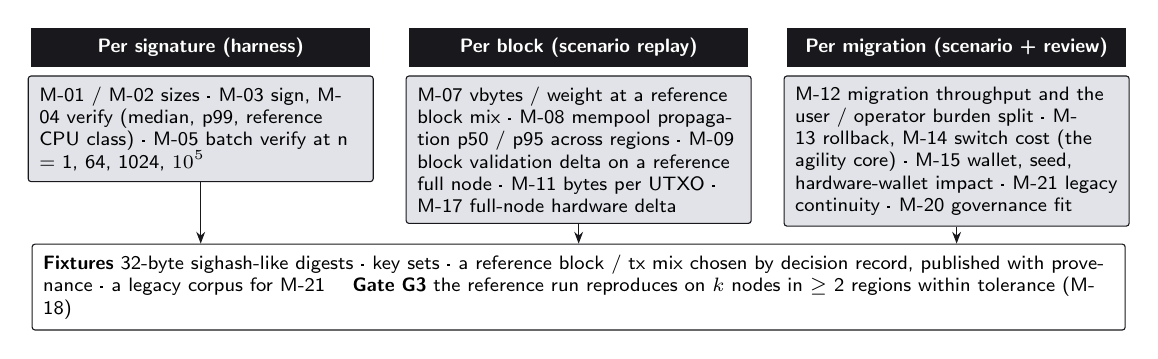
\begin{tikzpicture}[font=\scriptsize, box/.style={draw=bar,fill=lane,rounded corners=1pt,text width=4.1cm,align=left,inner sep=4pt}, hd/.style={fill=bar,text=white,font=\scriptsize\bfseries,text width=4.1cm,align=center,inner sep=3pt,minimum height=5mm}]
    \node[hd] (h1) at (0,0) {Per signature (harness)};
    \node[hd] (h2) at (4.8,0) {Per block (scenario replay)};
    \node[hd] (h3) at (9.6,0) {Per migration (scenario + review)};
    \node[box,below=1mm of h1] (b1) {M-01 / M-02 sizes \textperiodcentered{} M-03 sign, M-04 verify (median, p99, reference CPU class) \textperiodcentered{} M-05 batch verify at n = 1, 64, 1024, $10^5$};
    \node[box,below=1mm of h2] (b2) {M-07 vbytes / weight at a reference block mix \textperiodcentered{} M-08 mempool propagation p50 / p95 across regions \textperiodcentered{} M-09 block validation delta on a reference full node \textperiodcentered{} M-11 bytes per UTXO \textperiodcentered{} M-17 full-node hardware delta};
    \node[box,below=1mm of h3] (b3) {M-12 migration throughput and the user / operator burden split \textperiodcentered{} M-13 rollback, M-14 switch cost (the agility core) \textperiodcentered{} M-15 wallet, seed, hardware-wallet impact \textperiodcentered{} M-21 legacy continuity \textperiodcentered{} M-20 governance fit};
    \node[draw=bar,fill=white,rounded corners=1pt,text width=13.6cm,inner sep=4pt,align=left,below=2.5mm of b2.south,anchor=north] (ev) {\textbf{Fixtures} 32-byte sighash-like digests \textperiodcentered{} key sets \textperiodcentered{} a reference block / tx mix chosen by decision record, published with provenance \textperiodcentered{} a legacy corpus for M-21 \quad \textbf{Gate G3} the reference run reproduces on $k$ nodes in $\geq$ 2 regions within tolerance (M-18)};
    \foreach \b in {b1,b2,b3} \draw[-{Stealth[length=1.5mm]},bar] (\b.south) -- (\b.south |- ev.north);
  \end{tikzpicture}
  \end{center}
  \takeaway{Every performance number is a ratio against B-01 / B-02 on the same node. A Bitcoin reviewer gets deltas in the units they already use.}
\end{frame}

% ================================================================ 14 what stays outside
\begin{frame}{What Stays Outside Bitcoin Core's Remit --- and Outside BGIN's}
  \begin{columns}[T]
    \begin{column}{0.48\textwidth}
      {\small\textbf{Not asked of Bitcoin Core}}
      \begin{itemize}\small
        \item Adopting, endorsing or reviewing any scheme, output type or BIP because it appears in the register
        \item Deciding the fate of exposed-key or dormant coins
        \item Running or hosting the testbed --- node hosts are universities and neutral labs, funded transparently
        \item Sitting on the committee as ``Bitcoin'' --- seats are individuals with COI disclosure
      \end{itemize}
    \end{column}
    \begin{column}{0.48\textwidth}
      {\small\textbf{Not done by BGIN}}
      \begin{itemize}\small
        \item Chain endorsement, vendor scorecards, or a Q-day date
        \item New primitives or parameter sets --- NIST is the reference
        \item Prize adjudication --- the host's process; BGIN organizes the committee and testbed
        \item Policy decrees on transition design --- O4 is discussion input, recorded, not ruled
      \end{itemize}
    \end{column}
  \end{columns}
  \takeaway{The register asks Bitcoin engineers for one thing: that the Bitcoin deltas are measured the way a Core reviewer would measure them. That needs Bitcoin engineers writing the fixtures.}
\end{frame}

% ================================================================ 15 asks to bitcoin engineers
\begin{frame}{Three Asks to the Bitcoin Engineers in the Room}
  \begin{enumerate}\small
    \item \textbf{Technical-advisor seat, Bitcoin track} --- input on baselines, the reference block / tx mix, the M-15 wallet checklist, without winner-selection votes. COI form; nominations are open on the Discourse category.
    \item \textbf{Fixtures by pull request} --- the sighash-like corpus, the reference block mix and its provenance, the legacy corpus for M-21. The repository is public and every commit is signed and signed-off; a PR is the record.
    \item \textbf{A node, or a name} --- the node-host call opens at W3 (November): a reference full node in a university or neutral lab, in a region the testbed lacks. Or the name of the lab that should be asked.
  \end{enumerate}
  \par\vspace{2mm}
  {\small The committee's Bitcoin member seats (2--3, per the proposed composition) are the primary evaluation focus for the BTC-tx mapping. They are individuals, not projects.}
  \takeaway{Bitcoin's evidence is in the standard only if Bitcoin engineers put it there. Nothing in the process can substitute for that.}
\end{frame}

% ================================================================ SECTION 3
\sectiontitle{Session 2 \textperiodcentered{} 11:30--13:00}{Crypto Agility as a Governance Property; the NIST Migration Path}{Agility is harder than readiness and is what future-proofs the system. This session writes the agility and governance rows, hears the NIST signature migration path, and takes the W2 decisions.}

% ================================================================ 16 agility
\begin{frame}{Agility Is Harder Than Readiness --- Outcome O3}
  \lead{Evidence on the \textbf{mechanism of switching} --- hybrid and staged migration, scheme substitution cost, rollback, policy flexibility --- because the next migration is already certain and the primitive list will move again.}
  \begin{center}\scriptsize
  \begin{tabular}{@{}p{1.2cm}p{3.6cm}p{3.2cm}p{5.6cm}@{}}\toprule
    \textbf{Metric} & \textbf{What} & \textbf{Unit} & \textbf{How measured}\\ \midrule
    M-14 & Agility switch cost & time + coordination steps & scenario: swap scheme A to B under the proposed mechanism --- the core agility metric\\
    M-13 & Rollback cost & time + coordination steps & scenario: revert a staged migration\\
    M-12 & Migration throughput & keys / accounts per unit time & scenario; documents the user vs node-operator burden split\\
    M-21 & Legacy verification continuity & pass / fail + node cost & pre-migration signatures still verify after cutover\\ \bottomrule
  \end{tabular}
  \end{center}
  \takeaway{Design for the next migration now. A rushed cutover creates new incidents; a frozen profile goes stale. Both are scored.}
\end{frame}

% ================================================================ 17 governance property
\begin{frame}{Crypto Agility as a Governance Property --- Outcome O4}
  \pillar{0.31\textwidth}{Who upgrades first}{Node operators or users? M-12 makes the burden split explicit. On Bitcoin the answer differs by output type; on Ethereum by account model.}\hfill
  \pillar{0.31\textwidth}{The migration window}{The legitimate-owner-versus-attacker race is a governance question with a measurable shape: window length, what a wallet default does, what a rollback costs.}\hfill
  \pillar{0.31\textwidth}{Dormant and vulnerable assets}{Treatment of exposed-key and dormant funds is recorded as positions, scored under M-20 as a structured narrative --- discussion input, never a decree.}
  \par\vspace{2mm}
  {\small ``PQC-ready chain'' --- the definition M-22 scores against --- is the December deliverable (W4, SSR workshop). It has to be written so that ST/PP and wallet profiles can rotate algorithms without a fork-by-fork rewrite.}
  \takeaway{Agility written as a governance property is what lets the same rubric travel: competition $\rightarrow$ BGIN Standard $\rightarrow$ ISO/TC 307 $\rightarrow$ Japan's crypto-asset security criteria.}
\end{frame}

% ================================================================ 18 NIST path
\begin{frame}{The NIST Signature Migration Path --- What the Register Leans On}
  \lead{NIST is the algorithm and parameter authority for everything in scope; it is not a competition lane. Measurement-methodology cooperation is sought where appropriate.}
  \begin{itemize}\small
    \item \textbf{FIPS 204 ML-DSA}, \textbf{FIPS 205 SLH-DSA} --- standardized; S-01 and S-02.
    \item \textbf{FIPS 206 FN-DSA (Falcon)} --- draft; final expected late 2026 or 2027; S-03 is confirmed at the scope ruling.
    \item \textbf{SP 800-208} XMSS and LMS / HSS --- stateful hash-based; S-04 and S-05 with state handling scored.
    \item \textbf{ACVP / CAVP} wording is the T1 correctness gate for calibration tracks.
    \item Hybrid / composite signatures follow the \textbf{IETF LAMPS} direction (C-01).
    \item The on-ramp round-3 signature candidates are \textbf{out of scope by gate G1}.
  \end{itemize}
  \takeaway{The register tracks NIST's list; it never extends it. When the list moves, the agility metrics are what say whether a stack can follow.}
\end{frame}

% ================================================================ 19 decisions at W2
\begin{frame}{What Block 15 Decides --- the W2 Outputs}
  \begin{center}\scriptsize
  \begin{tabular}{@{}p{5.0cm}p{4.8cm}p{4.0cm}@{}}\toprule
    \textbf{Decision} & \textbf{Method} & \textbf{Lands as}\\ \midrule
    Committee seated (Phase A); chairs elected & nominations + COI forms; formal vote & COMMITTEE.md roster\\
    OUTCOMES O1--O6 ratified (if not at W1) & formal vote, quorum of half & decisions/ record\\
    Metric register v0 $\rightarrow$ v1; directions per metric & rough consensus on the PR & evaluation/METRICS.md\\
    Scheme-scope rulings: C-01 hybrid, C-02 P2QRH reference, S-04 non-SP-800-208 parameters, C-03 / C-04 / C-05 & formal vote per ruling & decisions/ records\\
    Open-benchmark model for calibration tracks & vote on decision 0001; recusals recorded & decisions/0001 accepted\\
    Open questions 1--5 assigned owners & conveners call it & workshop W2 record\\ \bottomrule
  \end{tabular}
  \end{center}
  \takeaway{Discuss on Discourse, record by pull request, rule by decision record. Every vote and every scope ruling gets an ADR.}
\end{frame}

% ================================================================ 20 open questions
\begin{frame}{The Open Questions That Need Owners Today}
  \begin{enumerate}\small
    \item Is the headline quantity \textbf{total overhead} or \textbf{migration speed}? The rubric decides the weights.
    \item Who must upgrade first --- \textbf{node operators or users} --- and how does M-12 reflect the burden split?
    \item How to score the \textbf{owner-versus-attacker race} during a migration window (M-20, track a)?
    \item Which \textbf{reference CPU class} and \textbf{reference tx mix / block} anchor M-03 to M-09? Decision record 0002 territory, with $k$ and the tolerance band.
    \item Are \textbf{consensus-layer} (ETH-cons) and \textbf{user-level} (BTC-tx, ETH-user) evidence scored on one rubric or two?
    \item For each metric, which attack class --- \textbf{on-spend, at-rest, on-setup} --- does it defend against?
  \end{enumerate}
\end{frame}

% ================================================================ 21 timeline
\begin{frame}{From This Room to the 2028 Award}
  \begin{center}
  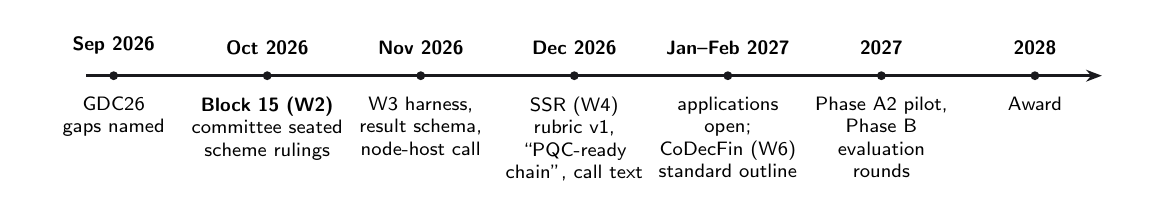
\begin{tikzpicture}[font=\scriptsize]
    \draw[line width=1pt,bar,-{Stealth[length=2mm]}] (0,0) -- (12.9,0);
    \foreach \x/\lab/\txt in {
      0.35/Sep 2026/{GDC26\\ gaps named},
      2.3/Oct 2026/{\textbf{Block 15 (W2)}\\ committee seated\\ scheme rulings},
      4.25/Nov 2026/{W3 harness,\\ result schema,\\ node-host call},
      6.2/Dec 2026/{SSR (W4)\\ rubric v1, ``PQC-ready\\ chain'', call text},
      8.15/Jan--Feb 2027/{applications open;\\ CoDecFin (W6)\\ standard outline},
      10.1/2027/{Phase A2 pilot,\\ Phase B evaluation\\ rounds},
      12.05/2028/{Award}}
      {\fill[bar] (\x,0) circle (1.6pt);
       \node[above=1.5mm,align=center,font=\scriptsize\bfseries] at (\x,0) {\lab};
       \node[below=1.5mm,align=center,text width=1.95cm] at (\x,0) {\txt};}
  \end{tikzpicture}
  \end{center}
  \par\vspace{1mm}
  \begin{center}\small
    Competition / evaluation $\rightarrow$ BGIN Standard $\rightarrow$ ISO/TC 307 $\rightarrow$ Japan's crypto-asset security criteria
  \end{center}
  {\scriptsize\color{soft} Dates are indicative until the host confirms the call. Between workshops: Discourse carries the discussion, PRs carry the record, decision records carry the rulings.}
  \takeaway{This morning can still change what the call asks teams to prove. SSR on 13 December is the next drafting stop.}
\end{frame}

% ================================================================ 22 engage
\begin{frame}{How to Engage}
  \begin{columns}[T]
    \begin{column}{0.55\textwidth}
      \begin{itemize}\small
        \item \textbf{Evaluation committee} --- draft call text, metrics and rubrics in Phase A; nominate via the issue template.
        \item \textbf{Technical advisor} --- Bitcoin / Ethereum / measurement input without winner votes.
        \item \textbf{Testbed node host} --- a university or neutral lab; contracting later; role separated from judging.
        \item \textbf{SSR workshop, 13 Dec} --- papers due 12 Oct; accepted papers feed the competition specification.
        \item \textbf{Submit / build} --- when the official call opens (planned 2027).
      \end{itemize}
    \end{column}
    \begin{column}{0.42\textwidth}
      \begin{center}\tiny
        \begin{tabular}{@{}>{\centering\arraybackslash}p{2.6cm}@{\hspace{3mm}}>{\centering\arraybackslash}p{2.6cm}@{}}
          \qrcode[height=1.6cm]{https://github.com/bgin-global/pqc-agility-competition} & \qrcode[height=1.6cm]{https://bgin.discourse.group/c/post-quantum-crypto-agility-competition/44} \\[0.5mm]
          \textbf{Repository} & \textbf{Discourse category} \\
          github.com/bgin-global/ pqc-agility-competition & bgin.discourse.group/c/ post-quantum-crypto-agility-competition/44
        \end{tabular}
      \end{center}
    \end{column}
  \end{columns}
  \takeaway{Discussion on Discourse; the repository is the record. Nothing is final until the committee ratifies it and the host publishes the call.}
\end{frame}

% ================================================================ CLOSE
{\setbeamertemplate{footline}{}
\begin{frame}[plain]
  \begin{tikzpicture}[remember picture,overlay]
    \fill[bar] (current page.north west) rectangle (current page.south east);
    \node[anchor=south,text=white,font=\Large\bfseries,text width=13.5cm,align=center,execute at begin node=\nohyph] at ([yshift=6mm]current page.center){The hard problem is deployment, evaluation, and migration governance.};
    \node[anchor=north,text=white,font=\small,text width=13.5cm,align=center,execute at begin node=\nohyph] at ([yshift=3mm]current page.center){Not selecting a new primitive. Not a date. Not an endorsement.};
    \node[anchor=north,text=soft,font=\small,text width=13.5cm,align=center,execute at begin node=\nohyph] at ([yshift=-9mm]current page.center){BGIN IKP Working Group \textperiodcentered{} Post-Quantum Crypto Agility Competition category on the BGIN Discourse \textperiodcentered{} github.com/bgin-global/pqc-agility-competition};
    \node[anchor=south east,inner sep=0] at ([xshift=-7mm,yshift=5mm]current page.south east){
\includegraphics[height=1.4cm]{bgin_logo.png}};
  \end{tikzpicture}
\end{frame}}

\end{document}
